% =====================================================================================================
%  Radiology: Artificial Intelligence -- Original Research
%  Focused paper: the counting mechanism. NOT a cut-down of paper/rsnai/main.tex, which is a naming
%  study. Every number here is read from docs/COUNTING_EVIDENCE.md (generated from the result JSONs),
%  docs/WRONG_LEVEL_COST_EVIDENCE.md, docs/WRONG_SITE_BURDEN_EVIDENCE.md, docs/SWEEP_TIME_EVIDENCE.md
%  and docs/SWEEP_PROTOCOL.md. Nothing is typed from memory. Arms still in flight are marked [PENDING]
%  with the arm's name rather than guessed.
%
%  Bibliography: the task text said \bibliography{../rsnai/refs}; from paper/focused/_drafts/ that path
%  does not resolve, so it is ../../rsnai/refs, which is the same file.
% =====================================================================================================
\documentclass[11pt,letterpaper]{article}
\usepackage[margin=1in]{geometry}
\usepackage[T1]{fontenc}
\usepackage{lmodern}
\usepackage{helvet}
\renewcommand{\familydefault}{\sfdefault}
\usepackage{setspace}
\usepackage{graphicx,booktabs,array,amsmath,xcolor,microtype}
\usepackage[labelfont=bf,font=small]{caption}
\usepackage{tikz}
\usepackage[numbers,sort&compress]{natbib}
\usepackage[hidelinks]{hyperref}
\setstretch{1.15}

\newcommand{\pc}[1]{#1\,\%}

\begin{document}

% ------------------------------------------------------------------------------------------------ TITLE
\begin{center}
{\Large\bfseries Making the Count Exact: Ordinal Vertebral Localization from Overlapping C-arm Exposures,\\ With No Learned Component in the Count\par}
\vspace{0.8em}
{\normalsize Gregory Schwing, MD, PhD\par}
\vspace{0.3em}
{\small Department of Neurosurgery, Wayne State University School of Medicine / Detroit Medical Center, Detroit, MI\par}
{\small \texttt{go2432@wayne.edu}\par}
\end{center}

\vspace{0.5em}
\noindent\textbf{Article type:} Original Research. \textbf{Main text:} about 3,400 words.
\textbf{Display items:} one figure, two tables.\\
\textbf{Conflicts of interest:} the author has a commercial interest in a level-confirmation product under
development.\\
\textbf{Data sharing:} every imaging source is public. The counting tool and the result files from which
Tables~\ref{tab:count} and \ref{tab:boxes} are generated are released with the code.

% ------------------------------------------------------------------------------------------------ ABSTRACT
\section*{Abstract}

\noindent\textbf{Background.} Wrong-level spine surgery persists under the Universal Protocol because the
protocol verifies a site that has been \emph{marked}, and a vertebral level has no mark. The level is
counted, in theatre, across several limited fluoroscopic fields, and each join between fields can be one
body off.

\noindent\textbf{Purpose.} To measure how exactly a target vertebra is reached by counting nodes along a
chain of overlapping fluoroscopic exposures, linked by image correlation restricted to the step the
protocol commanded, with no learned component participating in the count.

\noindent\textbf{Materials and Methods.} Retrospective study of public data. Sweeps were cut from labelled
long images: 801 abdominopelvic CTs, 76 whole-spine CTs, routine clinical CTs from a second institution
(522 reaching the sacrum, 204 holding C2), and held-out real lateral radiographs. Frames of a stated physical span were taken with a
commanded step and degraded independently. Consecutive frames were linked by normalized cross-correlation
restricted to within 0.6 of a vertebral body pitch of that step; nodes were indexed by ordinal from an
anchor, and the target was the $k$-th node. Nothing is fitted in the count, so no spine was withheld on a
model's account. The outcome was the share of walks placing the mark on the body truly $k$ from the anchor,
among walks whose target entered a field. \textbf{Every headline number uses the annotation's vertebra
boxes}; detector-box arms are reported separately.

\noindent\textbf{Results.} At three bodies of overlap from C2, 834 of 834 walks were exact on 76
whole-spine studies and 2,640 of 2,650 (\pc{99.62}) on 204 studies from a second institution. From the
sacrum, 6,214 of 6,229 (\pc{99.76}) were exact on all 801 abdominopelvic spines, and 7,168 of 7,228
(\pc{99.17}) at two bodies on 522 second-institution spines. Walks used 1.15 to 2.96 exposures. On real
radiographs, 95 of 95 walks on 16 spines were exact with the annotation's boxes and 95 of 95 with the
deployed film detector's boxes; from C2, 110 of 110 on 24 spines. On 79 cases scored with a render-trained
detector's boxes the same walks fell to 187 of 622 (\pc{30.06}), and the node the count started from was
the true sacrum on \pc{42.44} of walks.

\noindent\textbf{Conclusion.} Counting across overlapping exposures is exact and needs no network. The
residual risk is entirely in the vertebra boxes, and specifically in the anchor.

\medskip
\noindent\textbf{Abbreviations:} NCC = normalized cross-correlation.

% ------------------------------------------------------------------------------------------------ INTRO
\section*{Introduction}

The Universal Protocol verifies a mark. A vertebral level does not have one. Site marking works because a
limb, a side or an organ can be signed before induction and inspected at the time-out; a vertebral body
cannot be marked through the skin with the accuracy of a single segment, so the level is established after
incision, by counting on intraoperative images that show three or four bodies at a time. Chart review of
insured wrong-site cases judged the Universal Protocol would have prevented eight of 13 (\pc{62}) under
optimal conditions \citep{kwaan2006}, wrong-site events continued through the protocol era
\citep{stahel2010}, and the one study to assess site-verification protocols in the spine found they failed
to prevent about a third of cases \citep{longo2012}. The remedy the spine literature recommends, imaging
after exposure against a marked fixed structure \citep{devine2010}, is itself another count.

The residue is small per procedure and large per career. Half of responding neurosurgeons in two
independent surveys report at least one wrong-level operation \citep{mody2008,groff2013}. A prospectively
collected registry of 34,544 degenerative spine operations recorded \pc{0.12} (95\,\% CI 0.09--0.16), with
the thoracic spine highest at \pc{0.42} (CI 0.16--1.08), three times the lumbar and eight times the
cervical rate \citep{furuya2026}; self-report gives one in 3,110 \citep{mody2008}. Seventeen percent of
self-reported events led to legal action or settlement \citep{mody2008}, 55 of 68 litigated wrong-disc-level
cases ended in a payment \citep{goodkin2004}, the median indemnity for a surgical never event reported to
the National Practitioner Data Bank is \$75,220 \citep{bettis2026}, and the mean closed wrong-site claim in
a contemporary series was \$136,453 with spine surgery the commonest procedure \citep{tan2023}; England's
978 spinal-surgery negligence claims over five years were valued at \pounds535.5 million
\citep{machin2018}. The aggregate is bounded rather than counted: 127 reports of wrong surgery reached the
Joint Commission in 2024, nine wrong-level and seven of those spinal, through a voluntary system it states
captures a small fraction \citep{jc2024}, and NHS England recorded 185 wrong-site never events in one year
\citep{nhse2025}. The often-quoted \$1.3 billion is a 21-year cumulative for \emph{all} surgical never
events \citep{mehtsun2013}, not an annual wrong-site figure, and no defensible worldwide total exists in
the evidence assembled here.

What is spent avoiding the error shows what the error is worth. One quaternary centre placed 179
preoperative percutaneous gold fiducials over 38 months, 176 of them thoracic, at a mean of 51.9 minutes
and 183\,mGy each, purely to mark a level \citep{siminski2023}; at a hospital operating-room cost of
\$34--37 per minute before physician fees \citep{childers2018} that is roughly \$1,750--\$1,950 of staffed
procedural time per patient. Thoracic localization by fluoroscopic counting has been reported at about 15
minutes, falling to about three with a fiducial already in place \citep{mongardi2021,upadhyaya2012}, and
that fiducial costs 14.3 minutes of CT-suite time \citep{keil2024}.

Two observations organize what follows. First, surgeons do not classify vertebrae by morphology. They
count, down from C2 or up from the sacrum, and they disagree even on which structure to count --- the
pedicle for \pc{67} and the spinous process for \pc{49} of respondents in the thoracic spine
\citep{strong2021,mayer2008}. The intervention that matches the practice is therefore not a classifier that
asserts an identity, but a mechanism that makes the existing count exact across fields. Second, the
automated alternative in the literature imports identity rather than reading it: registering a preoperative
CT to the radiograph solves a six-degree-of-freedom pose and transfers the name from a human's reading of
the volume \citep{levelcheck2012,otake2015}. That is unavailable when no CT exists, and a miscounted
preoperative scan propagates onto the radiograph faithfully.

This study measures a third thing. Because the C-arm moves a commanded distance between exposures,
consecutive limited fields overlap by a known amount and link into one chain of vertebrae; the target is
the $k$-th node from an anchor, no network takes part, and the quantity produced is an ordinal rather than
a name.

% ------------------------------------------------------------------------------------------------ METHODS
\section*{Materials and Methods}

This retrospective study used public, de-identified data only; institutional review determined it not to be
human-subjects research.

\subsection*{Why an unconstrained correlation search fails on a spine}

The lateral spine is quasi-periodic. Vertebral bodies of similar size repeat at a pitch $p$ of about
34\,mm in the lumbar spine, so the normalized cross-correlation between the overlap bands of two
consecutive frames, as a function of axial shift $\Delta$, has a peak not only at the true displacement $d$
but also at $d\pm p$, $d\pm 2p$, and so on: a body matched against its neighbour agrees almost as well as a
body matched against itself. The margin between the true peak and its neighbour is small, and it is made
smaller by exactly the things that differ between two independently taken exposures --- gain, offset,
collimation, a small rotation, noise. When the alias wins, the two frames are joined one body off, every
node above the join shifts by one, and the resulting chain is a perfectly plausible consecutive spine, so
nothing downstream detects it. This is the documented dominant failure of automatic vertebral localization;
it accounted for all 47 failures in the original three-dimensional-to-two-dimensional registration study
\citep{otake2012fail}. It is also the surgeon's own error, reproduced by a machine.

\subsection*{Why restricting the search to the commanded step removes the competing peak}

The protocol does not move the C-arm an unknown distance. It commands a step $s$ --- one field span minus
two vertebral bodies --- and the executed move differs from $s$ by a small residual $e$, so the true
displacement is $d=s+e$. Restricting the NCC search to $|\Delta-s|\le 0.6\,p$ therefore excludes the
aliases outright rather than merely outranking them: the competing peaks sit at $d\pm p = s+e\pm p$, and
they enter a window of half-width $0.6\,p$ only if $|e|\ge 0.4\,p$, that is, only if the actual move erred
by more than about 14\,mm in the lumbar spine (Fig.~\ref{fig:mechanism}). The constraint is prior
information injected by the act of moving the C-arm a commanded distance; it is not read off the image, and
it does not weaken when the image does. Two consequences are built into the protocol handed to the
radiographer. Overlap is set at two bodies,
which is enough shared structure to place the peak and few enough frames that there are few links to get
wrong. And the last move is a full move or none: a final step shorter than half a body makes $s$ small, the
window around it admits $\Delta=0$ and $\Delta=p$ together, and the search is back in the situation the
restriction exists to prevent. The linker refuses steps under half a body for that reason.

\subsection*{Why an ordinal is a different and safer quantity than a name}

Naming a vertebra requires two things: a position in the column, and an alphabet that maps positions to
names. The alphabet is a property of the patient. A sixth lumbar vertebra, a thirteenth rib-bearing level
or a sacralized L5 shifts every name above the variant by one while leaving the column itself unchanged.
An ordinal requires only an anchor and the successor relation. The body four above the sacrum is the body
four above the sacrum whether it is called L2 or L3, so transitional anatomy cannot make the ordinal wrong;
it can only make a \emph{name} wrong. Nothing is fitted in an ordinal count, so there is no
training-distribution question for it, no spine has to be withheld for having been seen, and every scan
carrying the anchor was used --- 801 abdominopelvic spines, not the 120 a held-out naming evaluation
allows.

\subsection*{The algorithm, in the form required to reimplement it}

\begin{enumerate}\setlength\itemsep{1pt}
\item Place the anchor at the edge of the first field: the sacral promontory and S1 body at the bottom for
lumbar or thoracolumbar work, the odontoid and C2 body at the top for cervical or upper thoracic work.
Expose. Do not change field size or magnification for the rest of the sweep.
\item Move the C-arm toward the target by the commanded step $s$ = field span at the spine minus two
vertebral bodies, and expose again. Repeat until the target is in the field. Field span at the spine is
about 14, 19 and 20\,cm for a 9-inch intensifier, a 12-inch intensifier and a 30\,cm flat panel, and about
10\,cm collimated, given a mobile C-arm's fixed source-to-detector distance \citep{naik2022,ge_k170752}.
\item Obtain vertebra boxes in each frame from any detector. The count uses their positions only; their
classes are not read.
\item For each consecutive pair, compute NCC over the overlap band for $\Delta\in[s-0.6p,\,s+0.6p]$ and
take the argmax. Refuse the link if the commanded step was under $0.5p$.
\item Map the boxes of frame $i+1$ into frame $i$ by $\Delta$. A box pairs with the box of frame $i$ whose
centre lies within half a pitch of it; unpaired boxes beyond the leading edge become new nodes, appended in
order. The ordered union over all pairs is the chain.
\item Index the chain from the anchor node. Two anchor rules were evaluated: \emph{terminal}, in which the
anchor is the extreme node at the anchor edge of the first frame, and \emph{class}, in which a classifier
identifies the sacrum or C2 and the system refuses when no anchor is found. Every result below uses the
terminal rule; the class rule is [PENDING] (arms \emph{sacrum, CTSP, detector boxes, anchor = class} and
\emph{sacrum, films, film detector, anchor = class}).
\item The target is node $k$. Its position in the live frame follows from the accumulated translations.
\end{enumerate}

\subsection*{Data, sweep simulation, and boxes}

Serial sweeps of one patient exist in no public collection, so a sweep was cut from each labelled long
image: frames of a stated physical width, the step as above, each frame degraded independently by gain,
offset, gamma, a small rotation and scale, and a fitted film-noise model, so no two frames share pixels
exactly. Sources were 801 abdominopelvic CTs with per-level labels, 76 whole-spine CTs, a second
institution's public release of routine clinical CTs (522 of them reach the sacrum and 204 hold C2, and
the two sets overlap), and held-out real lateral radiographs (16 reaching the sacrum,
24 holding C2). Overlap was two or
three bodies as stated per arm.

Vertebra boxes came from the annotation in every arm except where the table says otherwise. Two
detector-box arms were run: a detector trained on renders, scored on the 79 cases held out from it, and the
deployed film detector on the 16 real-film spines. Because the count itself is not fitted, an
annotation-box arm is not a holdout question; a detector-box arm is, and is restricted to cases held out
from that detector.

\subsection*{Outcomes}

A walk from the anchor to a target at ordinal $k$ is \emph{exact} when the marked node is the body that is
truly $k$ from the anchor in the label sequence. \emph{Reached} walks are those whose target entered a
field before the image ran out; walks that did not reach are reported separately and are not counted as
errors, because they are a limitation of field rather than of counting. \emph{Anchor held} is the share of
walks whose starting node really was the anchor; it is a diagnostic and never a gate. Exposures are the
mean number of frames a walk consumed. Compute was measured per frame and per walk.
No hypothesis test was applied.

% ------------------------------------------------------------------------------------------------ RESULTS
\section*{Results}

\subsection*{Counting with the annotation's boxes}

Table~\ref{tab:count} gives every arm. Counting down from C2 on 76 whole-spine studies was exact on 832 of
834 walks at two bodies of overlap and on \textbf{834 of 834 at three}, from a mean of 2.24 exposures; the
two failures at two bodies fell in one study. On 204 studies from a second institution, 2,646 of 2,654
reached walks were exact at two bodies (\pc{99.70}) and 2,640 of 2,650 at three (\pc{99.62}), the misses
confined to two spines in each arm.

Counting up from the sacrum on all 801 abdominopelvic spines was exact on 6,234 of 6,255 reached walks at
two bodies (\pc{99.66}) and 6,214 of 6,229 at three (\pc{99.76}), the errors concentrated in six and five
spines. On 522 second-institution spines the figure was 7,168 of 7,228 (\pc{99.17}) from 2.96 exposures,
with 60 wrong walks in six spines. Walks that never reached their target were 97 and 123 of 6,352 on the
abdominopelvic spines and 168 of 7,396 on the second institution's, almost all of them the topmost labelled
body or a cervical level far above the sacrum.

Error is not uniform along the column, and it grows with the distance walked. From the sacrum on the
abdominopelvic spines, lumbar targets were exact \pc{99.73} of the time and thoracic targets \pc{95.45}; on
the second institution's spines, lumbar \pc{99.33}, thoracic \pc{97.41} and cervical \pc{83.84}. Counting down from C2 on the same
second-institution spines, the gradient runs the other way: cervical \pc{100}, thoracic \pc{99.71} and lumbar \pc{97.87} at two bodies
of overlap. Each anchor is most exact near itself.

On real lateral radiographs the count was exact on every walk: 95 of 95 on the 16 spines that reach the
sacrum, from 1.61 exposures, and 110 of 110 from C2 on 24 spines, from 1.15. Sixteen and 24 spines are few,
and the $n$ is stated beside each figure.

\subsection*{The residual risk is in the boxes, and specifically in the anchor}

Table~\ref{tab:boxes} holds the central comparison. On the 79 abdominopelvic cases held out from
the render-trained detector, walks with the annotation's boxes were exact on 618 of 618 reached walks
(\pc{100}). On the same cases with that detector's boxes, 187 of 622 were exact (\pc{30.06}), and the node
the count started from was the true sacrum on \pc{42.44} of walks. Raising overlap to three bodies did not
help --- \pc{28.66} exact, anchor held \pc{39.77} --- because more frames mean more boxes, not better ones.
By region, detector-box walks were exact \pc{39.29} of the time to lumbar targets and \pc{13.60} to
thoracic ones: the further the walk, the more chances a missing or spurious box has to shift the ordinal.

The mechanism of that collapse is the one the method is otherwise built to prevent. A missed box removes a
node and renames every body above it by one; a spurious box inserts one and does the same in the other
direction. The count is then internally consistent and wrong, which is the surgeon's own failure mode
reintroduced by a machine. The anchor is the worst place for it to happen, because an anchor error shifts
the entire chain. The fix follows from the diagnostic: identify the anchor by class rather than by taking
the terminal node of the first frame, and refuse the walk when no anchor is found. Those arms are
[PENDING].

With the deployed film detector on the 16 real-film spines, all 95 walks were exact from 1.47 exposures,
with the anchor held on \pc{93.68}. That the ordinal survived on every walk while the anchor diagnostic did
not hold on all of them is not explained here; on those films the terminal node and the annotated landmark
need not be the same body, and no arm has yet separated the two effects.

\subsection*{What the count costs, and what naming costs beside it}

Linking a walk took 0.10 to 0.29 seconds and decoding 0.0002 seconds, timed in the two large naming arms,
which run the same linker.
The counting arms load no network, so the encoder's 0.017--0.018 seconds per frame is a cost of naming, not
of counting. Against this, repositioning a mobile C-arm takes 36 to 49 seconds per move in the only
time-motion measurements available (46 and 49 seconds on test rigs; 41.0\,$\pm$\,30.9 and
36.4\,$\pm$\,33.2 seconds to reach a target view) \citep{matthews2007,desilva2018}, and physical
manipulation, not beam time, dominates it. A walk
of two to three exposures is therefore one to three minutes of C-arm work and under a second of computation.
For comparison, the only clinically translated automatic system reports 4.7 seconds per image on a 2012
graphics card and 17 to 72 seconds per case in its 2018 operating-room deployment
\citep{levelcheck2012,otake2015}.

Naming the same chains with the study's encoder and run-level head was correct on \pc{96.25} of 950 walks
on the abdominopelvic spines (lumbar \pc{94.98}, thoracic \pc{93.75}) and \pc{94.69} of 7,405 walks on the
second institution's (lumbar \pc{96.21}, thoracic \pc{91.58}, cervical \pc{80.35}). Naming is three to five
points below counting on the same sweeps, and the gap widens exactly where the alphabet is least certain.

% ------------------------------------------------------------------------------------------------ DISCUSSION
\section*{Discussion}

Counting is exact and needs no network. Across 76, 204, 801 and 522 spines the walk from an anchor to a
target placed the mark on the right body on \pc{99.17} to \pc{100} of reached walks, from two or three
exposures, with the annotation's boxes. The mechanism that makes it exact is not a model: it is the
restriction of the correlation search to the step the protocol commanded, which removes the periodic
column's competing peak from the search space rather than asking a score to outrank it.

The division of labour that follows is this paper's contribution. Counting produces an ordinal, and an
ordinal is safe under variant anatomy because it never chooses an alphabet. Naming produces a name, and a
name requires an alphabet the patient may not have; that is where the uncertainty lives, and it is a
per-spine decision rather than one classification per vertebra. The network's proper job is not to identify each
vertebra from its morphology but to decide which alphabet this spine is written in. When the operative plan
is stated relative to the anchor --- the $k$-th mobile segment above the sacrum --- counting alone suffices
and no network is needed at all.

The residual risk sits entirely in the boxes and predominantly in the anchor: the same 79 cases went from
\pc{100} exact to \pc{30.06} when a render-trained detector supplied the boxes, with the anchor correct on
\pc{42.44} of walks. A method whose accuracy is a function of one box must refuse when that box is absent,
and the arm that anchors by class rather than by terminal node is [PENDING]. Until it reports, the
deployable claim is narrower than the headline: the linking is solved, the detection is not.

This slots into the Universal Protocol as the site-marking step the spine has never had. Verification
enters the target level; the sweep places a digital mark on the body it counts to; the time-out compares
that mark's count against the surgeon's own, and a disagreement is resolved by rule rather than by
deference. It is assistance, not replacement, and its failure mode is auditable by eye: the chain of
overlapping images is a visible object, and a surgeon can see which two frames were joined where. That is
a different safety argument from a confidence score.

The deployment argument is architectural, not about speed: the compute is negligible either way, so
latency is not the case to make. The case is one model instead of two --- no
preoperative CT to register against, no optical tracker, no line of sight to maintain, no fiducial placed
in a CT suite the day before --- running on an embedded computer beside a C-arm the hospital already owns.
Community hospitals and ambulatory surgery centres operate without navigation suites, whose capital cost
was not measured here and is not claimed; what a registration system needs, a preoperative CT with a
correct human count on it, is absent in precisely the setting where the level is hardest to name.

\subsection*{Limitations}

The sweeps are simulated. Frames are cut from single long images and degraded independently, which
reproduces independent exposure, noise, rotation and scale between frames but not parallax between
exposures taken at different C-arm positions and not patient motion during the sweep. Both act on the
linking rather than on the count's arithmetic, and neither has been measured. No sweep has been performed on
a patient.

Every headline number uses the annotation's vertebra boxes and therefore measures the linker, not a
deployable system. The real-film arms are 16 and 24 spines. The second institution's release carries no
sixth-lumbar or thirteenth-thoracic class: the ordinal is indifferent to variant anatomy by construction,
but that indifference is an argument here, not a measurement on variant spines. Walks that did not reach
their target are excluded from the accuracy denominator, and both denominators are in
Table~\ref{tab:count}. One release-level label error sits inside the abdominopelvic errors. Three arms are still running and are marked [PENDING] rather than
estimated: anchoring by class on renders and on film, the C2-class anchor detector, and the needle
confirmation experiment, in which a metal instrument is re-imaged from the same or a slightly different
angle and localized on the map to confirm which body is being touched. Its section in the evidence brief
is empty, so nothing about it is reported.

% ------------------------------------------------------------------------------------------------ FIGURE
\begin{figure}[htbp]\centering
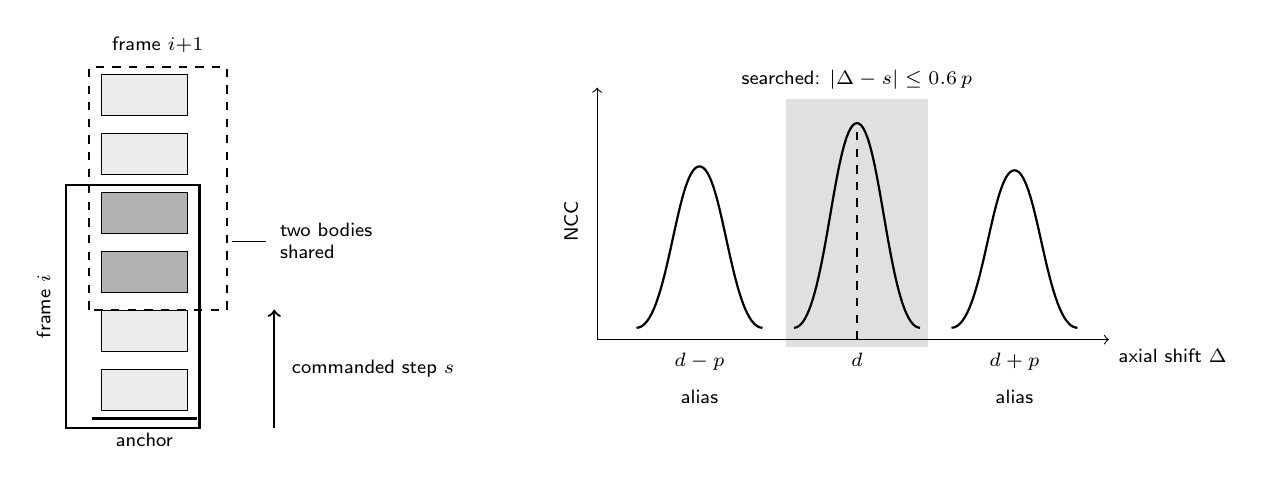
\begin{tikzpicture}[x=1cm,y=1cm]

% ---------------- left panel: two overlapping fields on one periodic column
\begin{scope}[shift={(0,0)}]
  \foreach \i in {0,...,5} {
    \draw[fill=black!8] (0,0.75*\i) rectangle (1.1,0.75*\i+0.52);
  }
  \foreach \i in {2,3} {
    \draw[fill=black!30] (0,0.75*\i) rectangle (1.1,0.75*\i+0.52);
  }
  \draw[very thick] (-0.12,-0.10) -- (1.22,-0.10);
  \node[font=\scriptsize,anchor=north] at (0.55,-0.16) {anchor};

  \draw[thick] (-0.45,-0.22) rectangle (1.25,2.86);
  \node[font=\scriptsize,anchor=south,rotate=90] at (-0.52,1.32) {frame $i$};

  \draw[thick,dashed] (-0.15,1.28) rectangle (1.60,4.36);
  \node[font=\scriptsize,anchor=south] at (0.72,4.42) {frame $i{+}1$};

  \draw[->,thick] (2.20,-0.22) -- (2.20,1.28);
  \node[font=\scriptsize,anchor=west] at (2.30,0.53) {commanded step $s$};

  \draw[-] (1.66,2.15) -- (2.10,2.15);
  \node[font=\scriptsize,anchor=west,align=left] at (2.15,2.15) {two bodies\\shared};
\end{scope}

% ---------------- right panel: correlation over axial shift
\begin{scope}[shift={(6.6,0.9)}]
  \fill[black!12] (2.1,-0.1) rectangle (3.9,3.05);
  \draw[->] (-0.3,0) -- (6.2,0) node[anchor=north west,font=\scriptsize] {axial shift $\Delta$};
  \draw[->] (-0.3,0) -- (-0.3,3.2);
  \node[font=\scriptsize,anchor=south,rotate=90] at (-0.42,1.5) {NCC};

  \draw[thick] (0.2,0.15) .. controls (0.6,0.15) and (0.7,2.2) .. (1.0,2.2)
                          .. controls (1.3,2.2) and (1.4,0.15) .. (1.8,0.15);
  \draw[thick] (2.2,0.15) .. controls (2.6,0.15) and (2.7,2.75) .. (3.0,2.75)
                          .. controls (3.3,2.75) and (3.4,0.15) .. (3.8,0.15);
  \draw[thick] (4.2,0.15) .. controls (4.6,0.15) and (4.7,2.15) .. (5.0,2.15)
                          .. controls (5.3,2.15) and (5.4,0.15) .. (5.8,0.15);

  \draw[dashed] (3.0,0) -- (3.0,2.75);
  \node[font=\scriptsize,anchor=north] at (1.0,-0.05) {$d-p$};
  \node[font=\scriptsize,anchor=north] at (3.0,-0.05) {$d$};
  \node[font=\scriptsize,anchor=north] at (5.0,-0.05) {$d+p$};
  \node[font=\scriptsize,anchor=south] at (3.0,3.05) {searched: $|\Delta-s|\le 0.6\,p$};
  \node[font=\scriptsize,anchor=north] at (1.0,-0.52) {alias};
  \node[font=\scriptsize,anchor=north] at (5.0,-0.52) {alias};
\end{scope}

\end{tikzpicture}
\caption{Left: consecutive fields share two bodies after a commanded step $s$. Right: correlation over
axial shift peaks at the true displacement $d$ and again at $d\pm p$, one body pitch away, because the
column repeats. Searching only within $0.6\,p$ of $s$ puts the aliases outside the search.}
\label{fig:mechanism}
\end{figure}

% ------------------------------------------------------------------------------------------------ TABLES
\begin{table}[htbp]\centering
\caption{Counting arms with the annotation's vertebra boxes. \emph{Reached} walks are those whose target
entered a field before the image ran out; the accuracy denominator is \emph{reached}, and both denominators
are given so either can be formed. \emph{Wrong} counts walks, with the number of distinct spines they fall
in; \emph{Exact} is of reached. Both abdominopelvic arms use all 801 spines. The anchor held on every walk in every arm here.}
\label{tab:count}
\footnotesize\setlength{\tabcolsep}{4.5pt}
\begin{tabular}{l r r r r r r}
\toprule
Arm & Spines & Walks & Reached & Exact & Exposures & Wrong (spines)\\
\midrule
C2, two bodies, whole-spine CT & 76 & 834 & 834 & \pc{99.76} & 1.99 & 2 (1)\\
C2, three bodies, whole-spine CT & 76 & 834 & 834 & \textbf{\pc{100}} & 2.24 & 0 (0)\\
C2, two bodies, second inst. & 204 & 2656 & 2654 & \pc{99.70} & 2.05 & 8 (2)\\
C2, three bodies, second inst. & 204 & 2656 & 2650 & \pc{99.62} & 2.27 & 10 (2)\\
\midrule
Sacrum, two bodies, abdominopelvic & 801 & 6352 & 6255 & \pc{99.66} & 1.98 & 21 (6)\\
Sacrum, three bodies, abdominopelvic & 801 & 6352 & 6229 & \pc{99.76} & 2.42 & 15 (5)\\
Sacrum, two bodies, second inst. & 522 & 7396 & 7228 & \pc{99.17} & 2.96 & 60 (6)\\
\midrule
Sacrum, two bodies, real radiographs & 16 & 95 & 95 & \pc{100} & 1.61 & 0 (0)\\
C2, real radiographs & 24 & 110 & 110 & \pc{100} & 1.15 & 0 (0)\\
\bottomrule
\end{tabular}
\end{table}

\begin{table}[htbp]\centering
\caption{Where the residual risk is. The first three rows are the same 79 abdominopelvic cases, held out
from the render-trained detector, scored with the annotation's boxes and with that detector's. The last two
are the same 16 real-film spines. \emph{Anchor held} is the share of walks whose starting node really was
the anchor. Every row anchors on the terminal node; anchoring by class is [PENDING].}
\label{tab:boxes}
\small
\begin{tabular}{l l r r r r}
\toprule
Arm (overlap) & Boxes & Walks & Reached & Exact of reached & Anchor held\\
\midrule
79 CT cases, two bodies   & annotation      & 625 & 618 & \pc{100}   & \pc{100}\\
79 CT cases, two bodies   & render detector & 625 & 622 & \pc{30.06} & \pc{42.44}\\
79 CT cases, three bodies & render detector & 625 & 621 & \pc{28.66} & \pc{39.77}\\
\midrule
16 real films, two bodies & annotation      &  95 &  95 & \pc{100} & \pc{100}\\
16 real films, two bodies & film detector   &  95 &  95 & \pc{100} & \pc{93.68}\\
\bottomrule
\end{tabular}
\end{table}

\clearpage
\bibliographystyle{unsrtnat}
\bibliography{../../rsnai/refs}

\end{document}
